%!TEX root = /Users/jakubkonka/Thesis/Thesis.tex
\chapter{Historical Context} % (fold)
\label{cha:literature}

\minitoc
\vspace{10mm}

\section{Heterogeneous Wireless Access Networks} % (fold)
\label{sec:heterogeneous_wireless_access_networks}
Over the last decade, the world of wireless and mobile communications has witnessed several major improvements \cite{ABC03}. The evolution of traditional 2$^\text{nd}$ Generation (2G) cellular systems, such as Global System for Mobile Communications (GSM), into 3$^{\text{rd}}$ Generation (3G) systems, such as Universal Mobile Telephone System (UMTS) or Code Division Multiple Access 2000 (CDMA2000), has drastically improved the cellular coverage worldwide, and provided basic mobile Internet access. At the same time, IEEE 802.11-based Wireless Local Area Network (WLAN) solutions have emerged as the predominant high-speed wireless Internet access at airports, in hotels or even at home.

With the introduction of advanced mobile phones, more commonly referred to as smartphones, the wireless users can finally take advantage of both the coverage offered by 3G cellular access network and the high-speed Internet access offered by WLANs. Whenever the smartphone is in close proximity to a WLAN hot spot, it automatically switches from 3G to WLAN mode for faster data access. However, this only works when either the WLAN hot spot provides free access, or is within the user's subscription; for example, as part of the monthly data allowance plan with a local wireless access operator. Moreover, this solution lacks the support for session continuity, and does not provide any intelligence when switching from one access network to another. For instance, although the WLAN hot spot is by definition deemed to offer faster data rates, this does not necessarily translate into higher Quality of Service\footnote{Definition of QoS \cite{XiaoQoS08}} (QoS). In fact, it might be just the contrary, especially in a very crowded hot spot area where the users run very bandwidth intensive applications such as video or music streaming, or even on-line gaming. Under such circumstances, trying to make a Voice over IP (VoIP) phone call using Skype can be nigh impossible \cite{Wisely4gWLAN09}. Therefore, the decision to switch from one network to another should not only consider the availability of a particular wireless access network (say, WLAN) but also the offered QoS for the best user experience.
\begin{figure}[ht]
    \centering
    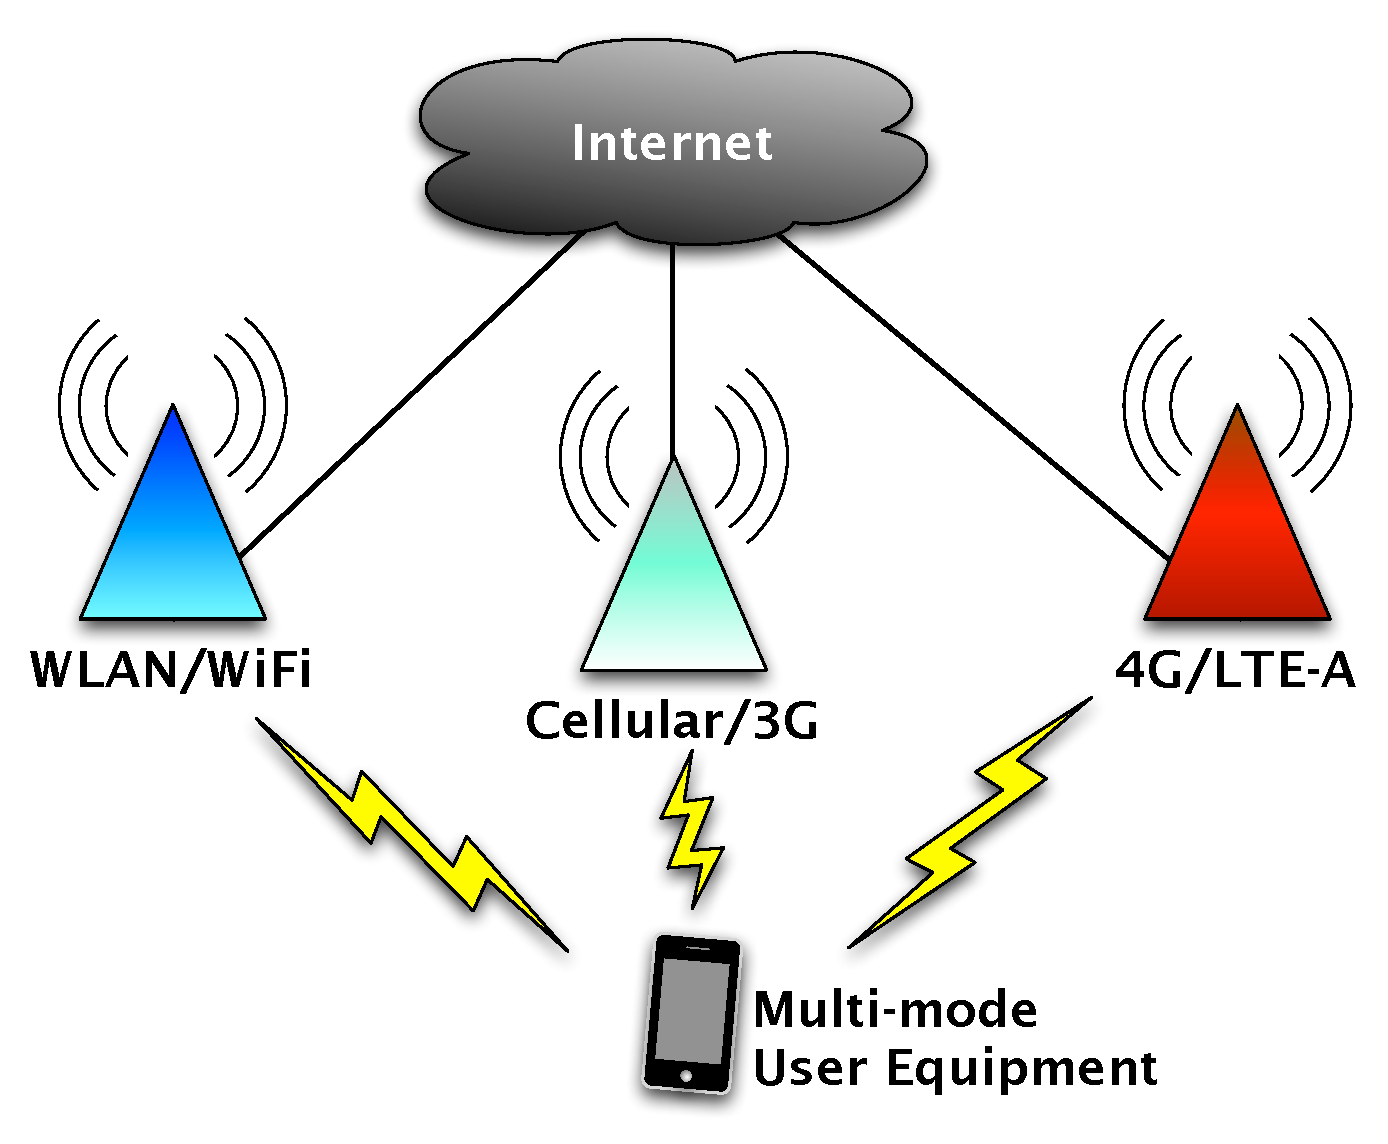
\includegraphics[width=3.5in]{Introduction/Figures/heterogeneous}
    \caption{Heterogeneous wireless access network}
    \label{fig:ch1_heterogeneous}
\end{figure}

In the advent of 4$^{\text{th}}$ Generation (4G) wireless systems, such as Worldwide Interoperability for Microwave Access (WiMAX) and Long Term Evolution Advanced (LTE-A), the wireless users will be able to choose from an even wider variety of different wireless access technologies \cite{HossainBeaubrun09, HossainTalebiFard09}. This, together with the industry's drive to have an all-IP-based traffic, gives rise to the concept of a \emph{heterogeneous wireless access network}. The heterogeneous wireless access network spans different wireless access technologies integrated into one network to provide wireless and mobile users with the requested multimedia services and QoS. The connection to the network will be available through the introduction of multi-mode user equipment; i.e., a device, similar to a smartphone, which integrates all or some of the wireless technologies included in the heterogeneous wireless access network (Figure~\ref{fig:ch1_heterogeneous}).

The heterogeneous wireless access network will possess many advantages over the contemporary wireless networking solution. From the users' perspective, different coverage and QoS characteristics of each of the included wireless access technologies will lead to the ability to seamlessly connect at any time, at any place, and to the access technology which offers the most optimal quality available. This is referred to as \emph{Always Best Connected} networking paradigm \cite{ABC03}, and will be introduced in more detail in the following Section~\ref{sec:always_best_connected_networking_paradigm}. From the network operators' perspective, on the other hand, the integration of wireless access technologies will allow for more efficient usage of the network resources, and might be the most economic way of providing both universal coverage and broadband access \cite{HossainBeaubrun09}. 
\begin{figure}[ht]
    \centering
    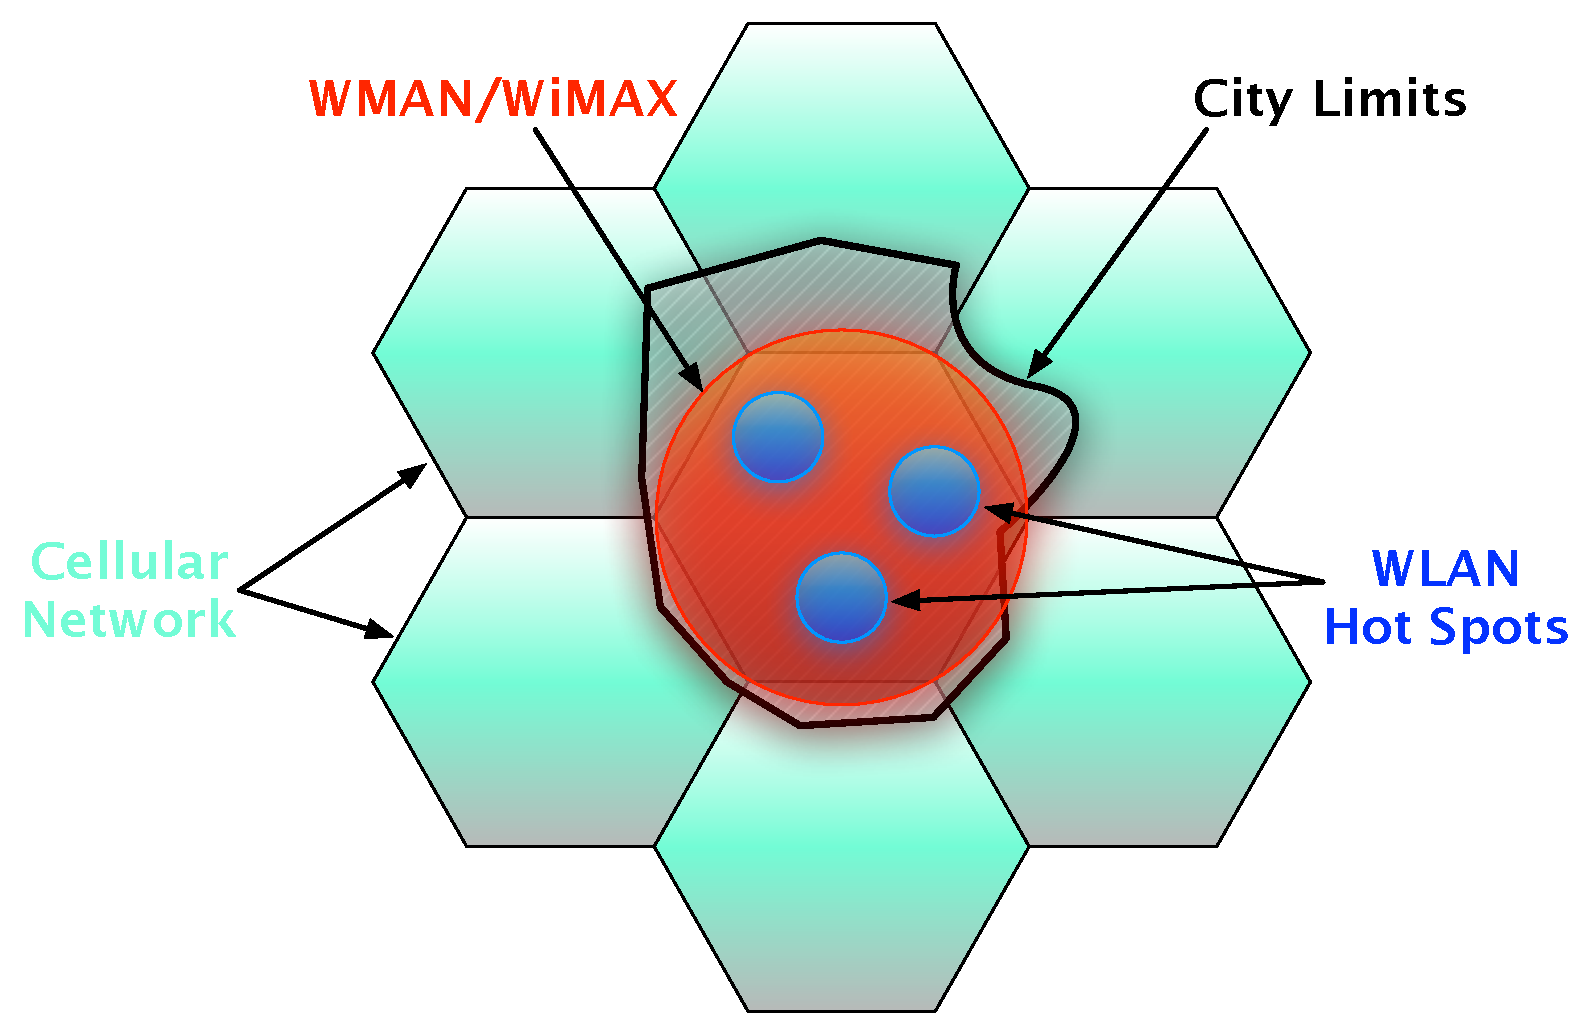
\includegraphics[width=4in]{Introduction/Figures/wireless_city}
    \caption{Enhanced wireless coverage and broadband access}
    \label{fig:ch1_wireless_city}
\end{figure}
Figure~\ref{fig:ch1_wireless_city} shows how a heterogeneous wireless access network can provide enhanced wireless coverage and broadband access across the entire city area. In the example, WLAN hot spots are used as a localised high-speed Internet access; WiMAX is used as a Wireless Metropolitan Area Network (WMAN), covering nearly the $\sfrac{3}{4}$ of the city area, and providing wireless broadband access; and the cellular network, which could be based on 3G or LTE-A, is used as a Wireless Wide Area Network (WWAN), and delivers medium speed wireless access inside as well as outside the city. The overlap of wireless access technologies provides potentially better network resources management, and also high-speed and high quality Internet access inside as well as outside the city limits.
% section heterogeneous_wireless_access_networks (end)

\section{Always Best Connected Networking Paradigm} % (fold)
\label{sec:always_best_connected_networking_paradigm}
As briefly mentioned in the previous section, \emph{Always Best Connected (ABC)} networking paradigm assumes that a wireless user is: (1) ``always'' connected to the Internet, and (2) uses the ``best'' access technology available \cite{ABC03}. ``Always'' can be understood as being able to utilise all wireless access technologies available at any time, while ``best'' implies that when a particular technology is being chosen, several factors such as user preferences, application requirements, network coverage, etc., are considered in order to make the most optimal selection possible (Figure~\ref{fig:ch1_abc}).
\begin{figure}[ht]
    \centering
    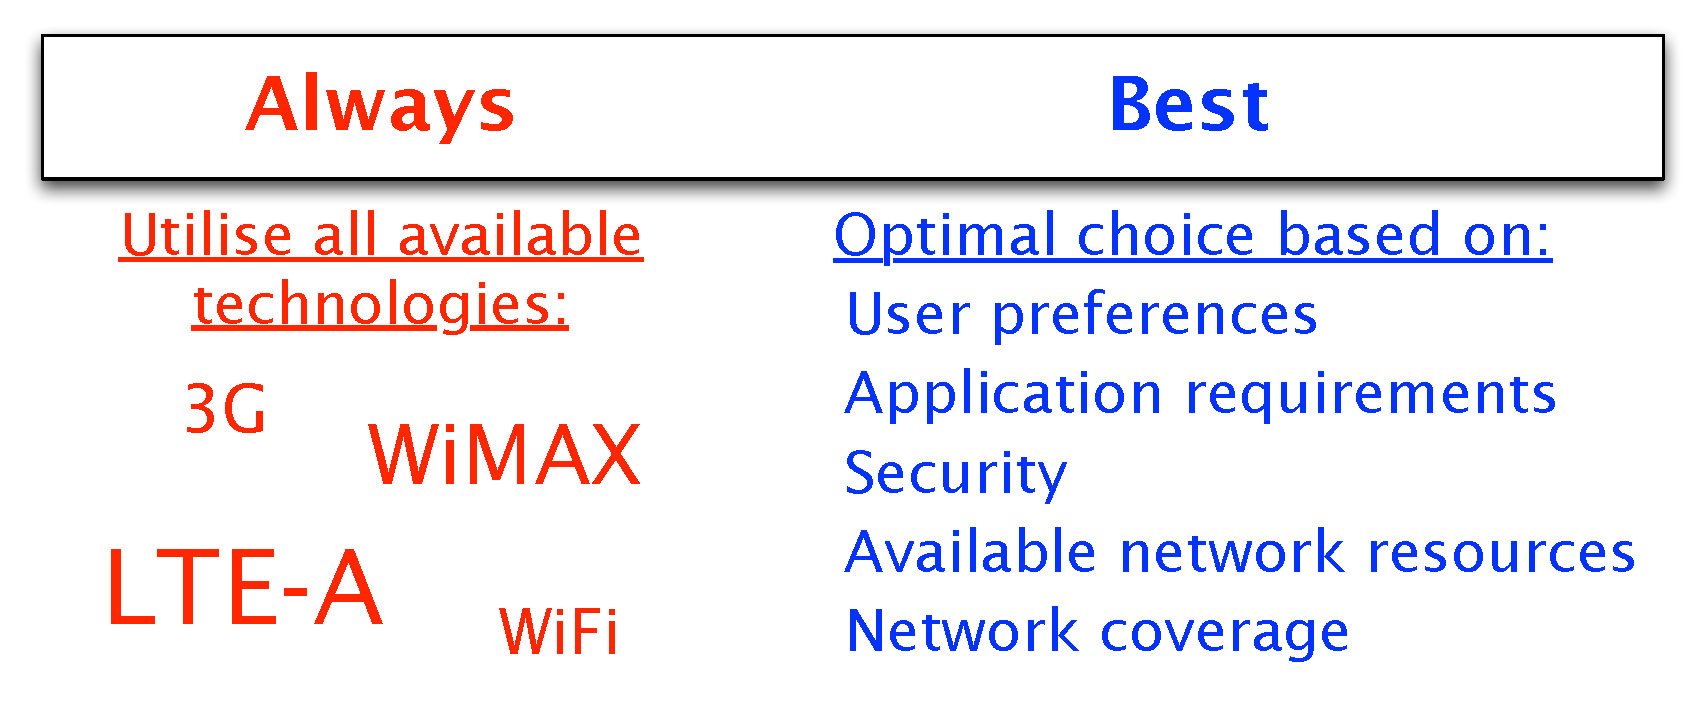
\includegraphics[width=4in]{Introduction/Figures/abc}
    \caption{The essence of ABC networking paradigm}
    \label{fig:ch1_abc}
\end{figure}

Furthermore, the paradigm emphasises seamless information delivery and extensive mobility support. In other words, the changes in the communications environment should affect the user as little as possible, even when they are ``on the move.'' Therefore, should the user move from the coverage area of one access technology to another, the initiated vertical handover\footnote{VHO is a special type of a handover which is executed when mobile equipment moves across different wireless access technologies \cite{HossainBeaubrun09}.} (VHO) should be as non-disrupting for the user as possible; i.e., the session continuity should be maintained at all times, regardless of the access technology currently used.

Thus, it is clear that network selection plays a vital role in the successful operation of the ABC solution.

% section always_best_connected_networking_paradigm (end)

\section{Intelligent Network Selection} % (fold)
\label{sec:intelligent_network_selection}
Over the last decade, several papers have explored the problem of intelligent network selection in heterogeneous wireless access networks. Wang and Kuo provide an up-to-date survey of the mainstream approaches to the network selection problem covering: utility and game theory, fuzzy logic, multiple attribute decision making, combinatorial optimization, and Markov chains \cite{LushengKuo2013}. Liu \emph{et al.}, propose an algorithm for optimal network selection which mainly aims at optimizing energy consumption of the user equipment \cite{Liu2009}. Espi~\emph{et al.} present a machine learning approach to network selection; in particular, the authors utilize a Hopfield neural network to solve the underlying optimization problem \cite{Espi10}. Antoniou \emph{et al.}, and Charilas \emph{et al.}~model the problem as a noncooperative game between wireless access networks with the aim of obtaining the best possible trade-off between the efficiency and the available capacity of networks, while, at the same time, satisfying the requested quality by the subscribers \cite{Antoniou07, Charilas08}. Ormond \emph{et al.}~propose an algorithm for cost-oriented and performance-aware network selection that maximizes consumer surplus \cite{OrmondCS106, OrmondCS206}. Niyato \emph{et al.}~propose two algorithms based on evolutionary game theory for a network selection mechanism which performs intelligent load balancing so that network congestion and performance degradation can be avoided \cite{Niyato09}. Addtionally, the same authors model the user churning behavior in heterogeneous wireless access networks using evolutionary game theory \cite{NiyatoHossainConf2008}. Khan \emph{et al.}~model the problem as a procurement second-price sealed-bid auction where network operators bid for the right to service the subscriber's request \cite{Khan110, Khan210}. Zhu \emph{et al.}~build upon the work reported in~\cite{Niyato09}, and explore the dynamics of network selection, using Bayesian evolutionary game theory, in an environment where subscribers have only limited (incomplete) information about each others preferences \cite{ZhuNiyato2010}. Finally, Irvine \emph{et al.}~propose a market-based framework called the Digital Marketplace where network operators compete in a variant of a procurement first-price sealed-bid auction for the right to transport the subscriber's requested service over their infrastructure \cite{DMLeBodic00, DMIrvine01, DMIrvine02}.
% section intelligent_network_selection (end)

% chapter literature (end)
